\chapter{Distributed Arithmetic}

Distributed Arithmetic is used to design bit-level(bit-serial) architectures for vector-vector multiplications.
Distributed Arithmetic replaces the multiplication operations in vector-vector multiplications with ROM lookups. It reorders and mixes the multiplications such that the arithmetic becomes 'distributed' throughout the structure.

The most computationally expensive operation in a LSTM cell is MatMul(matrix-vector multiplication) as observed from the profiling of the algorithm. Matrix-vector multiplication can be converted to vector-vector multiplication by representing the matrix as a column vector of rows or vice versa.

\section{Conventional Distributed Arithmetic}
Consider a simple inner product between two vectors $C$ and $X$ of length $N$.

\begin{equation}\label{eqn:eq1}
Y = C.X = \sum_{i=0}^{N-1} c_ix_i 
\end{equation}
where $c_i$'s are $M$-bit constants and $x_i$'s are coded as $W$-bit 2's complement numbers. The most significant bit in the 2's complement format represents the sign of the number while the rest of the bits have weights in power of two. The value of $W$-bit $x_i$ is given by : 

\begin{equation}\label{eqn:eq2}
x_i = -x_{i,W-1} + \sum_{j=1}^{W-1} x_{i, W-1-j}2^{-j}
\end{equation}
Substituting value of $x_i$ in \eqref{eqn:eq1}
\begin{equation}\label{eqn:eq3}
\begin{split}
Y &= \sum_{i=0}^{N-1} c_i  (-x_{i,W-1} + \sum_{j=1}^{W-1} x_{i, W-1-j}2^{-j}) \\
  &= -\sum_{i=0}^{N-1} c_ix_{i, W-1} + \sum_{j=1}^{W-1} (\sum_{i=0}^{N-1} c_ix_{i, W-1-j})2^{-j}
    \end{split}
\end{equation}
Let $C_j$'s be defined as
\begin{equation}
C_{W-1-j} = \sum_{i=0}^{N-1} c_ix_{i, W-1-j}
% \end{equation}
\quad (j\neq0), \, 
% \begin{equation}
C_{W-1} = - \sum_{i=0}^{N-1} c_ix_{i, W-1}
\end{equation}

\begin{equation}
Y = \sum_{j=0}^{W-1} C_{W-1-j}2^{-j}
\end{equation}
We have redistributed the arithmetic by interchanging the summing order of $i$ and $j$ in \eqref{eqn:eq3}

The terms $C_j$($2^N$ possible values) can be precomputed and stored in a read-only memory(ROM) since $C_j$'s depend on $x_{i,j}$'s. Note that this implies that a ROM of size $2^N$ has to be used.
An input address of $N$ bits ($x_{0,j}, x_{1,j}, x_{2,j} ..., x_{N-1,j}$) is used to retrieve the precomputed $C_j$ value. By addressing the ROM and accumulating the outputs, the inner product can be calculated in $W$ clock cycles.
So we have reduced the computations from $O(N)$ multiplications to $O(N-1)$ additions and right shift operations. There exists a trade off between computational complexity and memory here which will be exploited again in ROM Decomposition.
\begin{figure}[h]
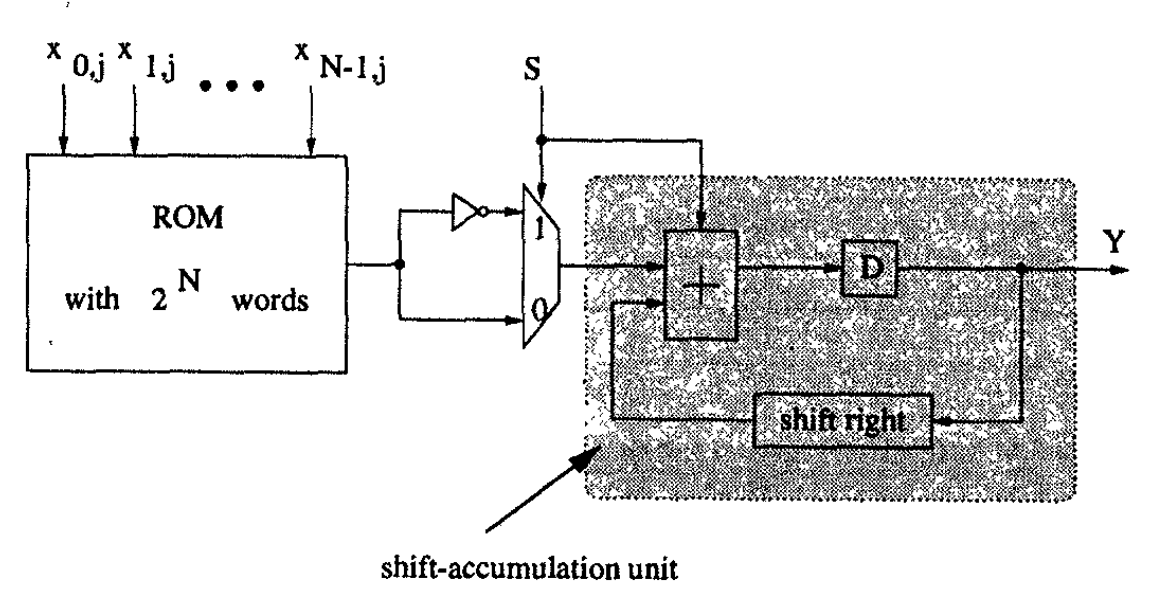
\includegraphics[scale=0.35]{images/da.png}
\end{figure}
Figure % figure number here
shows a typical architecture for computing inner product of two length-$N$ vectors using Distributed Arithmetic. The shift-accumulator is a bit-parallel carry-propagate adder that adds the ROM output to the previous adder output. The control signal $S$ is 1 when $j = W-1$ and 0 otherwise to invert the ROM output in order to calculate $C_{W-1}$. This inversion is achieved with the help of the MUX and the inverter. The result is accumulated in the adder after $W$ clock cycles($j=0$ to $j=W-1$).

\begin{center}
% \begin{tabular}{ |c|c|c|c|c| }
\begin{tabular}{ |>{\centering\arraybackslash}m{1cm}|>{\centering\arraybackslash}m{1cm}|>{\centering\arraybackslash}m{1cm}|>{\centering\arraybackslash}m{1cm}|>{\centering\arraybackslash}m{4cm}| }
\hline
$x_{0,j}$ & $x_{1,j}$ & $x_{2,j}$ & $x_{3,j}$ & ROM\\
\hline
0 & 0 & 0 & 0 & 0 \\
\hline
0 & 0 & 0 & 1 & $c_3$\\
\hline
0 & 0 & 1 & 0 & $c_2$\\
\hline
0 & 0 & 1 & 1 & $c_2+c_3$\\
\hline
0 & 1 & 0 & 0 & $c_1$\\
\hline
0 & 1 & 0 & 1 & $c_1+c_3$\\
\hline
0 & 1 & 1 & 0 & $c_1+c_2$\\
\hline
0 & 1 & 1 & 1 & $c_1+c_2+c_3$\\
\hline
1 & 0 & 0 & 0 & $c_0$ \\
\hline
1 & 0 & 0 & 1 & $c_0+c_3$\\
\hline
1 & 0 & 1 & 0 & $c_0+c_2$\\
\hline
1 & 0 & 1 & 1 & $c_0+c_2+c_3$\\
\hline
1 & 1 & 0 & 0 & $c_0+c_1$\\
\hline
1 & 1 & 0 & 1 & $c_0+c_1+c_3$\\
\hline
1 & 1 & 1 & 0 & $c_0+c_1+c_2$\\
\hline
1 & 1 & 1 & 1 & $c_0+c_1+c_2+c_3$\\
\hline
\end{tabular}
\end{center}




\section{ROM Decomposition}
\begin{figure}[h]
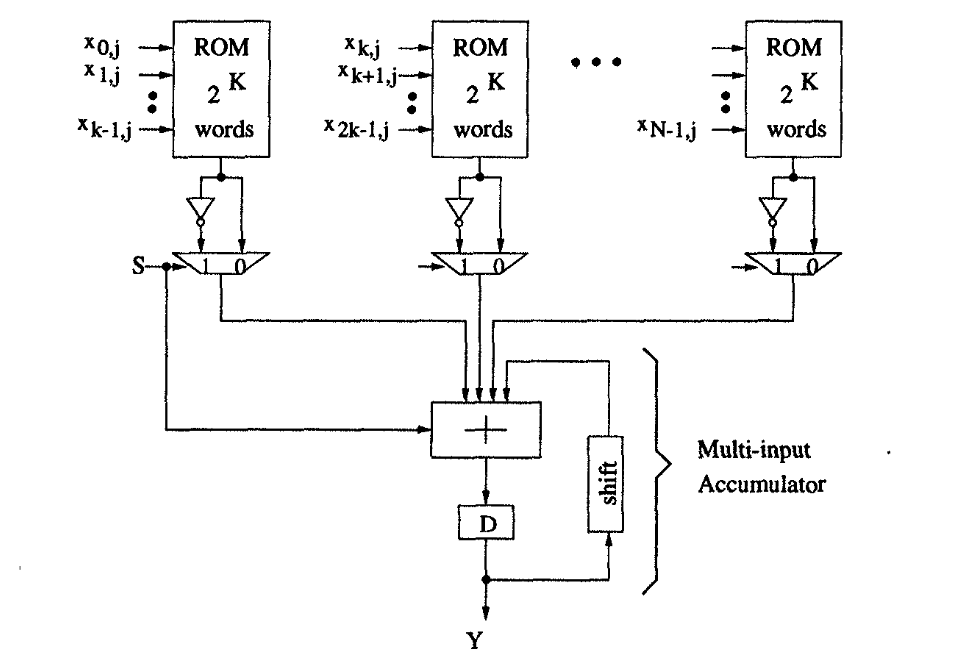
\includegraphics[scale=0.4]{images/da_decom.png}
\end{figure}
The ROM size of distributed arithmetic increases exponentially with the vector size $N$($2^N$) which along with the access time can bottleneck the speed of the whole system. The ROM size and access time can be improved by trading off the size with computational complexity of the accumulator.
The ROM size of the conventional DA and OBC based DA increases exponentially with the vector size $N$ ($2^N$ in conventional DA and $2^{N-1}$ in OBC based DA). When the ROM size is large, the ROM access time can limit the speed of the system. Hence, decreasing the ROM size is a very significant issue.

ROM decomposition provides a way to decrease the ROM size by trading off the ROM size with computational complexity. This can be achieved by dividing the $N$ address bits of the ROM into $N/K$ groups of $K$ bits effectively dividing or decomposing the ROM of size $2^N$ into $N/K$ ROMs of size $2^K$. This reduction in ROM size is at the cost of a multi-input accumulator to add the $N/K$ ROM outputs.
The total ROM size is now $(N/K)2^K$ which is a linear function of $N$ as opposed to an exponential increase.



\section{Offset Binary Coding}
Offset Binary Coding(OBC) based DA can reduce the ROM size from $2^N$ to $2^N-1$.
We write $x_i$ as
\begin{equation}\label{eqn:eq5}
\begin{split}
x_i &= \frac{1}{2}[x_i-(-x_i)]\\
    &= \frac{1}{2}[ -(x_{i, W-1}-\overline{x_{i, W-1}}) + \sum_{j=1}^{W-1}(x_{i, W-1-j} -\overline{x_{i, W-1-j}})2^{-j} - 2^{-(W-1)}]
\end{split}
\end{equation}
where $-x_i$ is
\begin{equation}
-x_i = -\overline{x_{i, W-1}} + \sum_{j=1}^{W-1}\overline{x_{i, W-1-j}}2^{-j} + 2^{-(W-1)}
\end{equation}
Define $d_{i,j}$ as
\begin{equation}\label{eqn:eq6}
d_{i,j} =
\begin{cases}
x_{i,j} - \overline{x_{i,j}},\ for \  j\neq W-1\\
-(x_{i, W-1} - \overline{x_{i, W-1}}),\ for\ j=W-1
\end{cases}
\end{equation}
Rewrite \eqref{eqn:eq5} using \eqref{eqn:eq6}
\begin{equation}\label{eqn:eq7}
x_i = \frac{1}{2}[\sum_{j=0}^{W-1}d_{i, W-1-j}2^{-j} - 2^{-(W-1)}]
\end{equation}
From \eqref{eqn:eq7} and \eqref{eqn:eq1}
\begin{equation}\label{eqn:eq8}
\begin{split}
Y &= \sum_{i=0}^{N-1}c_i[\frac{1}{2}(\sum_{j=0}^{W-1}d_{i, W-1-j}2^{-j} - 2^{-(W-1)})]\\
  &= \sum_{j=0}^{W-1}(\sum_{i=0}^{N-1}\frac{1}{2}c_id_{i,W-1-j})2^{-j} - (\sum_{i=0}^{N-1}\frac{1}{2}c_i)2^{-(W-1)}
\end{split}
\end{equation}
Define $D_j$
\begin{equation}
D_j = \sum_{i=0}^{N-1}\frac{1}{2}c_id_{i,W-1-j},\ for\ j=0\ to\ W-1
\end{equation}
and $D_{extra}$
\begin{equation}
D_{extra} = \sum_{i=0}^{N-1}\frac{1}{2}c_i
\end{equation}
Substituting $D_j$'s and $D_{extra}$ into \eqref{eqn:eq8}
\begin{equation}
Y = \sum_{j=0}^{W-1}D_{W-1-j}2^{-j} + D_{extra}2^{-(W-1)}
\end{equation}

\begin{center}
% \begin{tabular}{ |c|c|c|c|c| }
\begin{tabular}{ |>{\centering\arraybackslash}m{1cm}|>{\centering\arraybackslash}m{1cm}|>{\centering\arraybackslash}m{1cm}|>{\centering\arraybackslash}m{1cm}|>{\centering\arraybackslash}m{5cm}| }
\hline
$x_{0,j}$ & $x_{1,j}$ & $x_{2,j}$ & $x_{3,j}$ & ROM\\
\hline
0 & 0 & 0 & 0 & $-(c_0+c_1+c_2+c_3)/2$\\
\hline
0 & 0 & 0 & 1 & $-(c_0+c_1+c_2-c_3)/2$\\
\hline
0 & 0 & 1 & 0 & $-(c_0+c_1-c_2+c_3)/2$\\
\hline
0 & 0 & 1 & 1 & $-(c_0+c_1-c_2-c_3)/2$\\
\hline
0 & 1 & 0 & 0 & $-(c_0-c_1+c_2+c_3)/2$\\
\hline
0 & 1 & 0 & 1 & $-(c_0-c_1+c_2-c_3)/2$\\
\hline
0 & 1 & 1 & 0 & $-(c_0-c_1-c_2+c_3)/2$\\
\hline
0 & 1 & 1 & 1 & $-(c_0-c_1-c_2-c_3)/2$\\
\hline
\hline
\hline
1 & 0 & 0 & 0 & $(c_0-c_1-c_2-c_3)/2$\\
\hline
1 & 0 & 0 & 1 & $(c_0-c_1-c_2+c_3)/2$\\
\hline
1 & 0 & 1 & 0 & $(c_0-c_1+c_2-c_3)/2$\\
\hline
1 & 0 & 1 & 1 & $(c_0-c_1+c_2+c_3)/2$\\
\hline
1 & 1 & 0 & 0 & $(c_0+c_1-c_2-c_3)/2$\\
\hline
1 & 1 & 0 & 1 & $(c_0+c_1-c_2+c_3)/2$\\
\hline
1 & 1 & 1 & 0 & $(c_0+c_1+c_2-c_3)/2$\\
\hline
1 & 1 & 1 & 1 & $(c_0+c_1+c_2+c_3)/2$\\
\hline
\end{tabular}
\end{center}
The contents of the ROM have inverse symmetry as observed from the lookup table. This symmetry can be exploited to reduce the number of possible combinations by a factor of 2 reducing the ROM size by half.
\begin{figure}[h]
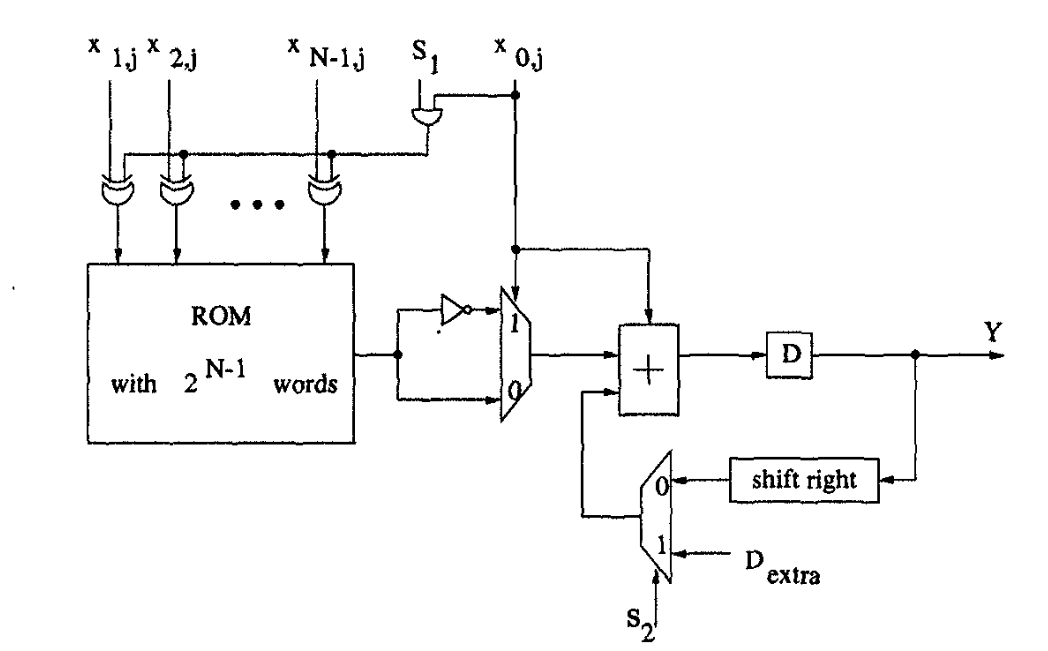
\includegraphics[scale=0.35]{images/da_obc.png}
\end{figure}

% figure number here
Figure shows a typical architecture for computing inner product of two length-$N$ vectors using OBC based DA. The architecture is mostly the same as conventional DA.

Control signal $S_2$ is 1 when $j=0$ and 0 otherwise providing the initial value $D_{extra}$ to the shift-accumulator. The XOR gates are used to select the correct address. The MUX after the ROM inverts the ROM output depending on the sign bit.


\section{Applying Distributed Arithmetic to LSTM}
% refer lstm equations
Refer to LSTM cell equations 
A simplified version can be written as $f(Wx+b)$ where $f$ is a non-linear activation function. The $Wx+b$ part can be optimized using DA. Write $W$ as
\begin{equation}
W = [w_0, w_1, w_2, w_3 ..., w_N-1]
\end{equation}
where $w_i$'s are column vectors of $W$ and x is a column vector.
So $Wx$ can be written as 
\begin{equation}
Wx = [w_0.x, w_1.x, w_2.x, w_3.x ..., w_N-1.x]^\top
\end{equation}
